\documentclass[10pt,leqno,aspectratio=169,presentation]{beamer} %handout
\usepackage[utf8]{inputenc}
%\usepackage{polski}
\usepackage{arydshln,ragged2e,lmodern,lipsum,multirow,multicol,bm,bbold}
\usepackage{graphicx,graphics,color,xcolor,colortbl,dsfont,caption}
\usepackage{natbib}
\usepackage[bars]{beamerthemetree}
\definecolor{UniBlue}{RGB}{83,121,170}
\definecolor{UniBlue2}{RGB}{75,47,87}
\usepackage[outdir=./]{epstopdf}
\usepackage{booktabs}

\usetheme{metropolis}
\usecolortheme{crane}


\setbeamertemplate{frame footer}{ 
\includegraphics[width=.12\textwidth]{Slides/logo_solo.png}}
\beamersetleftmargin{.25in}
\beamersetrightmargin{.25in}

\AtBeginSection{\frame{
\begin{center}
{\LARGE \insertsectionhead}
\end{center}
}}

\newcommand{\aheader}[2]{\action<#1-|alert@#1>{#2}}
\newcommand{\hiddencell}[2]{\action<#1->{#2}}

\definecolor{CiteBlue}{RGB}{50,120,200} % Bright blue
\let\oldcitet\citet
\renewcommand{\citet}[1]{\textcolor{CiteBlue}{{\oldcitet{#1}}}} % Bold + blue
\let\oldcitep\citep
\renewcommand{\citep}[1]{\textcolor{CiteBlue}{{\oldcitep{#1}}}} % Bold + blue
%---------------------------------------------------------------------------
\begin{document}


\title{Shocks and income inequality}

\author{Oleg Gurshev {\tiny(FAME$\mid$GRAPE)}  \\
Lucas van der Velde {\tiny (FAME$\mid$GRAPE, Warsaw School of Economics)}}
\date{\vspace{6pt} \centering  
\includegraphics[width=.33\textwidth]{Slides/logo_solo.png} \\ \footnotesize{EFES, Paris, 2025}}


% Title page
\begin{frame}
    \titlepage
\end{frame}

% Intro

\begin{frame}{Motivation}
\begin{enumerate}
    \item<1-> Motivation:
    \begin{itemize}
        \item<1-> Absence of empirical evidence on how shocks (US, domestic) to supply and demand contribute to income inequality and (so far) limited understanding of the US shocks and their possible effects in that context.
        \item<1-> Lack of evidence on how supply and demand shocks affect inequality.
        \item<1-> Contrast between domestic and international (US) shocks.
    \end{itemize}
    \item<2-> Goal:
    \begin{itemize}
        \item<2-> To study the dynamics of income inequality in response to US and domestic shocks.
    \end{itemize}
    \item<3-> Contribution and novelties:
    \begin{itemize}
        \item<3-> Standardized estimation of supply and demand shocks for several countries.
        \item<3-> Gini based on admin data (high quality data on labor earnings for computation of inequality measures)
        \item<3-> Relatively diverse open economy sample geographic.
    \end{itemize}
\end{enumerate}
\end{frame}


% Preview of results
\begin{frame}{Preview of findings}
    \begin{itemize}
        \item \textbf{Demand shocks}. US demand shocks cause inequality to rise abroad ($\uparrow$ Gini abroad between 0.5\% and 1\%). Domestic shocks feature similar behavior.
        \item \textbf{Supply shocks}. Both US and domestic shocks are not as persistent, but generally tend to reduce inequality (it's very modest though).
        \item \textbf{US vs domestic shocks}. US demand shocks generate stronger impact. Less clear for supply shocks (different signs, and not too robust)
        \item \textbf{Gender}. Income inequality grows faster for men, than for women (domestic demand shock only).
    \end{itemize}
\end{frame}

\begin{frame}{Related literature}
    \begin{enumerate}
    \item Role of the US and its domestic changes to output and labor market vis-a-vis the world\\
    {\footnotesize \citet{carrillo2020inquiry, Fink2015, kose2003, Kose2012, kose2017global, levchenko2020tfp, ramey2016macroeconomic}.}
    \item Shocks and inequality: \\ {\footnotesize \citet{andersen2023monetary, holm2021transmission, cloyne2020monetary, mumtaz2017impact, amberg2022five}}.
    \item Impact of monetary shocks on Gini: \\ {\footnotesize \citet{coibion2017innocent, Davtyan2017, furceri2018effects}}.
\end{enumerate}

Closest study - \citet{furceri2018effects} - JIMF.

% It would be nice if you can state the holes in the literature, and not just list the studies (during the presentation!, not here) 
\end{frame}
% Data
\begin{frame}{Data I - overview}
\begin{enumerate}
    \item \textbf{Shock computation and LPs}

    \only<2>{
\begin{itemize}
    \item Quarterly series: unemployment and real output growth (for shocks, per each country + US).
    \item Annual series: NBER, Fraser Institute, UNCTAD, \citet{Gygli2019} (for robustness controls during LP).
\end{itemize}
}

\medskip
    \item \textbf{Inequality measures}% (Gini) - panel for LPs
\only<3>{ 
\begin{itemize}
    \item Global Repository of Income Dynamics (GRID) by \citet{guvenen2022global}.
    \item Key advantages: (i) constructed using detailed administrative data, (ii) provides better coverage than similar open source databases (OECD, Luxembourg Income Study).
    \item Coverage of admin data used for Gini: ages 25-55, yearly gross earnings (i.e., base salary, overtime compensation, performance and seasonal bonuses, paid vacations, paid sick leaves, and severance payments).
    \item Sample: Canada, Denmark, France, Germany, Italy, Mexico, Norway, Spain, and Sweden.
    \item Also use Gini for subpopulations (gender).
\end{itemize}}
\end{enumerate}
\hspace{1em}Scope: 1990-2019 (time series+panel).
\end{frame}

% Data - descriptive stats of Gini
\begin{frame}{Data II - Gini}
    \begin{table}[H]
\captionsetup{justification=raggedright, singlelinecheck=false}
    \centering
    \caption{Availability of Gini data from GRID.}
    \begin{tabular}{l c c c c}
    \toprule
       Country & Scope & mean Gini & mean Gini (M) & mean Gini (F) \\
    \midrule
       Canada   & 1990-2019  & 0.41 (0.01) & 0.40 (0.02) & 0.38 (0.01) \\ 
       Denmark  & 1990-2016  & 0.28 (0.01) & 0.27 (0.02) & 0.25 (0.01) \\ 
       France   & 1991-2016  & 0.34 (0.00) & 0.34 (0.01) & 0.32 (0.00) \\ 
       Germany  & 2001-2016  & 0.40 (0.01) & 0.36 (0.02) & 0.39 (0.01) \\ 
       Italy    & 1990-2016  & 0.36 (0.02) & 0.34 (0.02) & 0.35 (0.02) \\ 
       Mexico   & 2005-2019  & 0.56 (0.00) & 0.57 (0.00) & 0.54 (0.01) \\ 
       Norway   & 1993-2017  & 0.33 (0.01) & 0.31 (0.02) & 0.32 (0.01) \\ 
       Spain    & 2005-2018  & 0.40 (0.01) & 0.39 (0.02) & 0.39 (0.01) \\ 
       Sweden   & 1990-2016  & 0.30 (0.01) & 0.28 (0.01) & 0.28 (0.01) \\ 
    \midrule
       \multicolumn{1}{l}{N} & \multicolumn{4}{l}{217} \\
    \bottomrule
    \end{tabular}
    
    \vspace{0.2cm}
    \raggedright\footnotesize Note: standard deviations in parenthesis, all data are annual.
\end{table}
\end{frame}

\begin{frame}{Evolution of Gini I}
    \begin{center}
    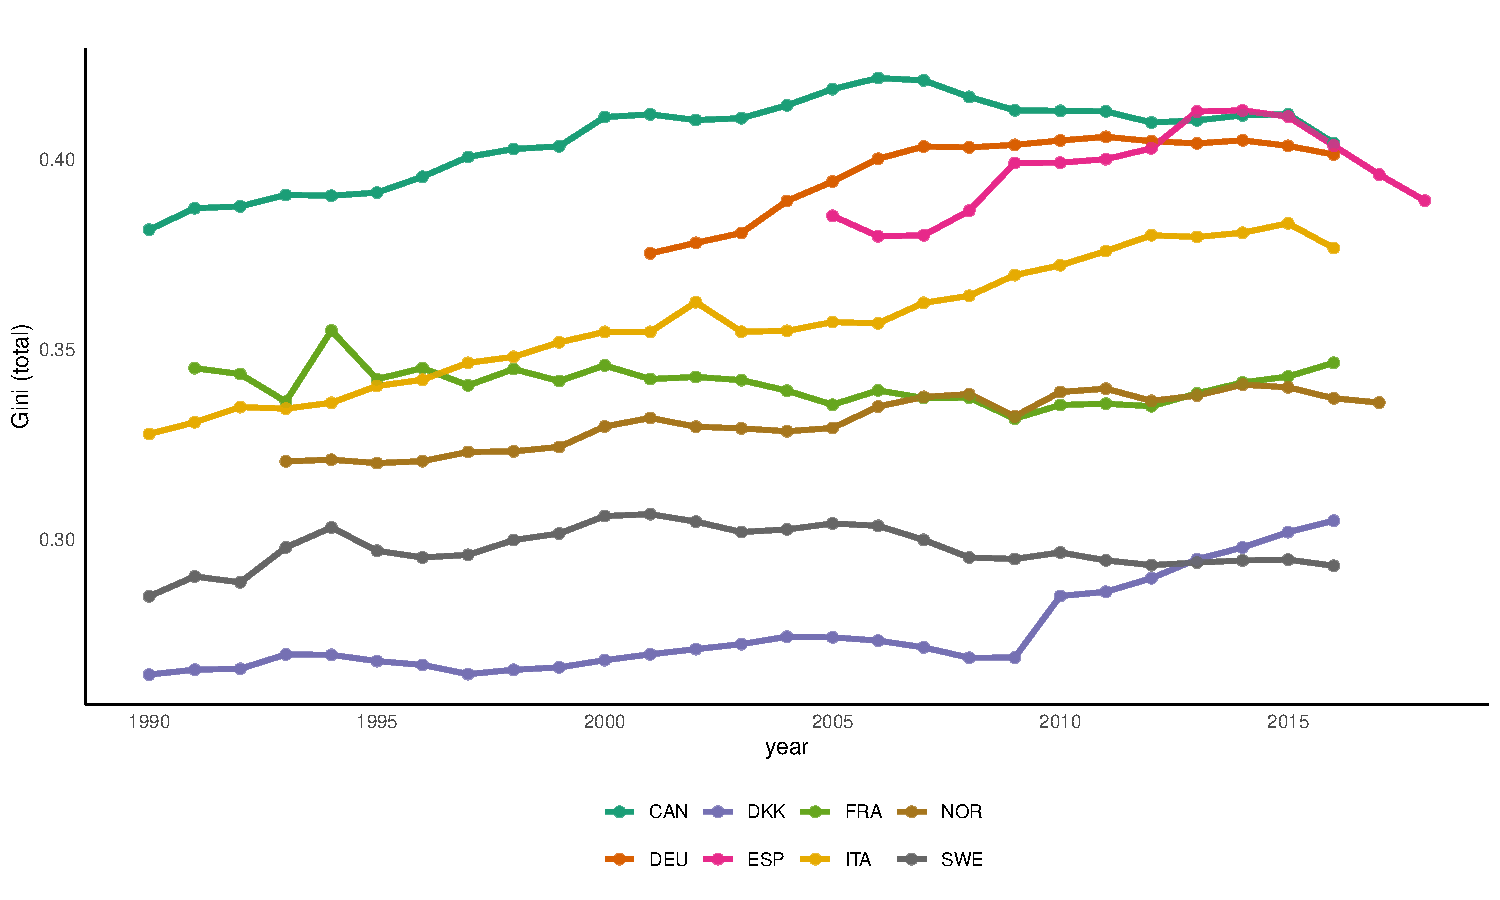
\includegraphics[width=0.80\textwidth]{Slides/Gini_no_MEX.pdf}
    \vspace{0.2cm} % Small vertical space
    \begin{minipage}{0.85\textwidth}
    \footnotesize
    Note: Mexico is omitted to improve readability.
    \end{minipage}
\end{center}
\end{frame}

\begin{frame}{Evolution of Gini II}
    \begin{center}
    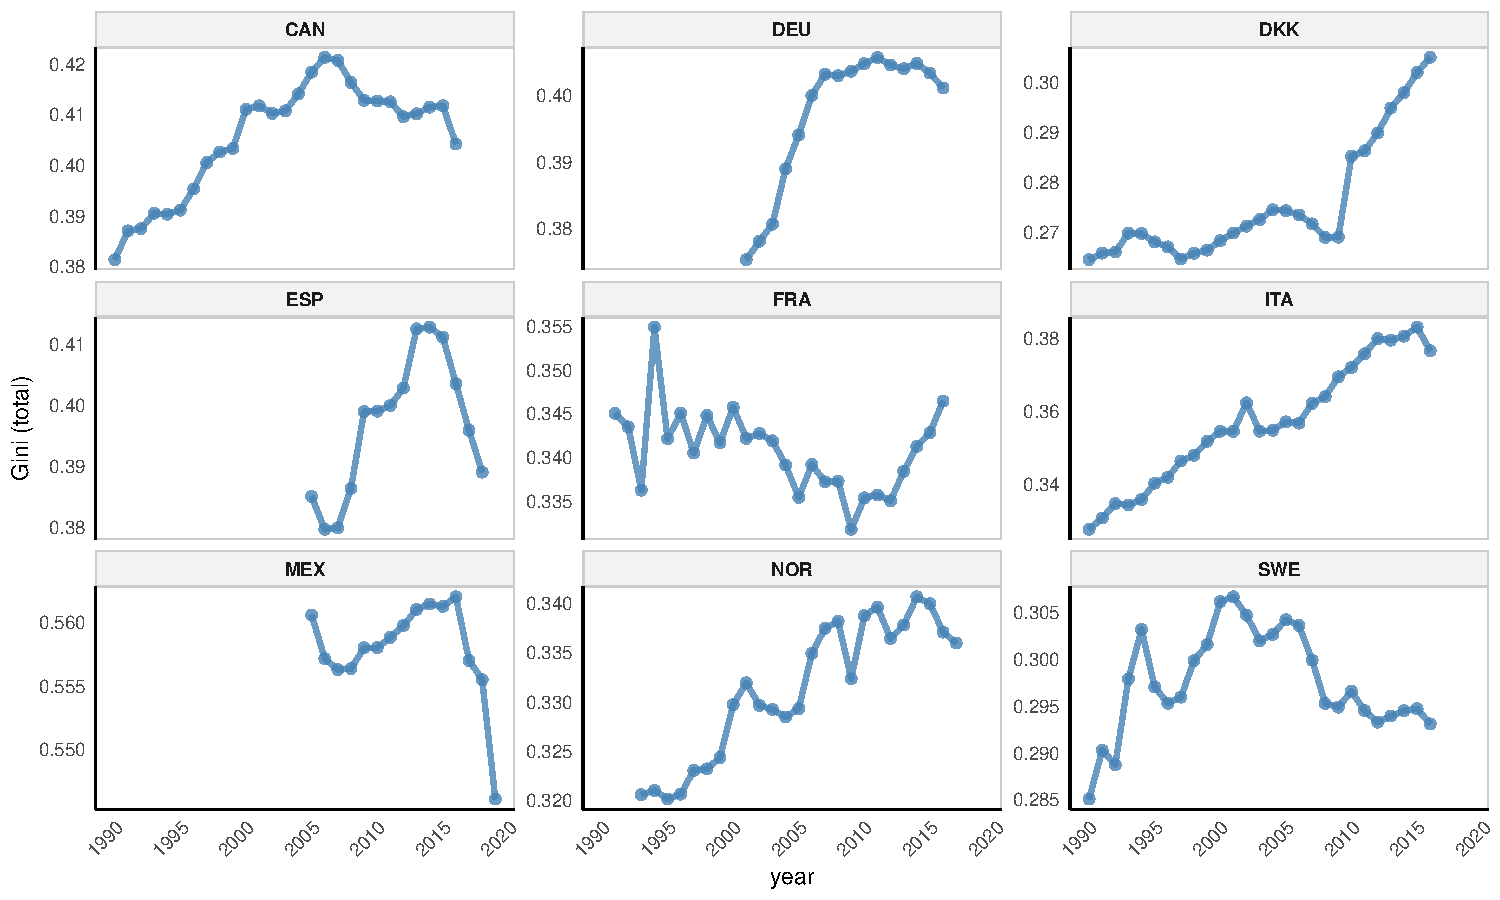
\includegraphics[width=0.85\textwidth]{Slides/Gini_with_MEX_facet.pdf}
    \vspace{0.2cm} % Small vertical space
\end{center}
\end{frame}

% Method
\begin{frame}{Methodology I - shock estimation}
\label{vAR}
For each country, we estimate shocks using long-run restrictions in the spirit of Blanchard-Quah \\
            (demand shocks have no long-run impact on output).

Key findings:
        \begin{itemize}
            \item Demand shocks are persistent (beyond 20 quarters).
            \item There are patterns for pairwise correlations across countries (Germany-France-Italy).
        \end{itemize}
Checks:
        \begin{itemize}
            \item IRFs patterns + visual inspection of disturbances.
            \item Orthogonality between the two shocks (within country correlation).
        \end{itemize}
\hyperlink{LRvar}{\beamerbutton{VAR algebra}}
\end{frame}

\begin{frame}{IRFs - positive shocks to supply and demand}
\begin{center}
    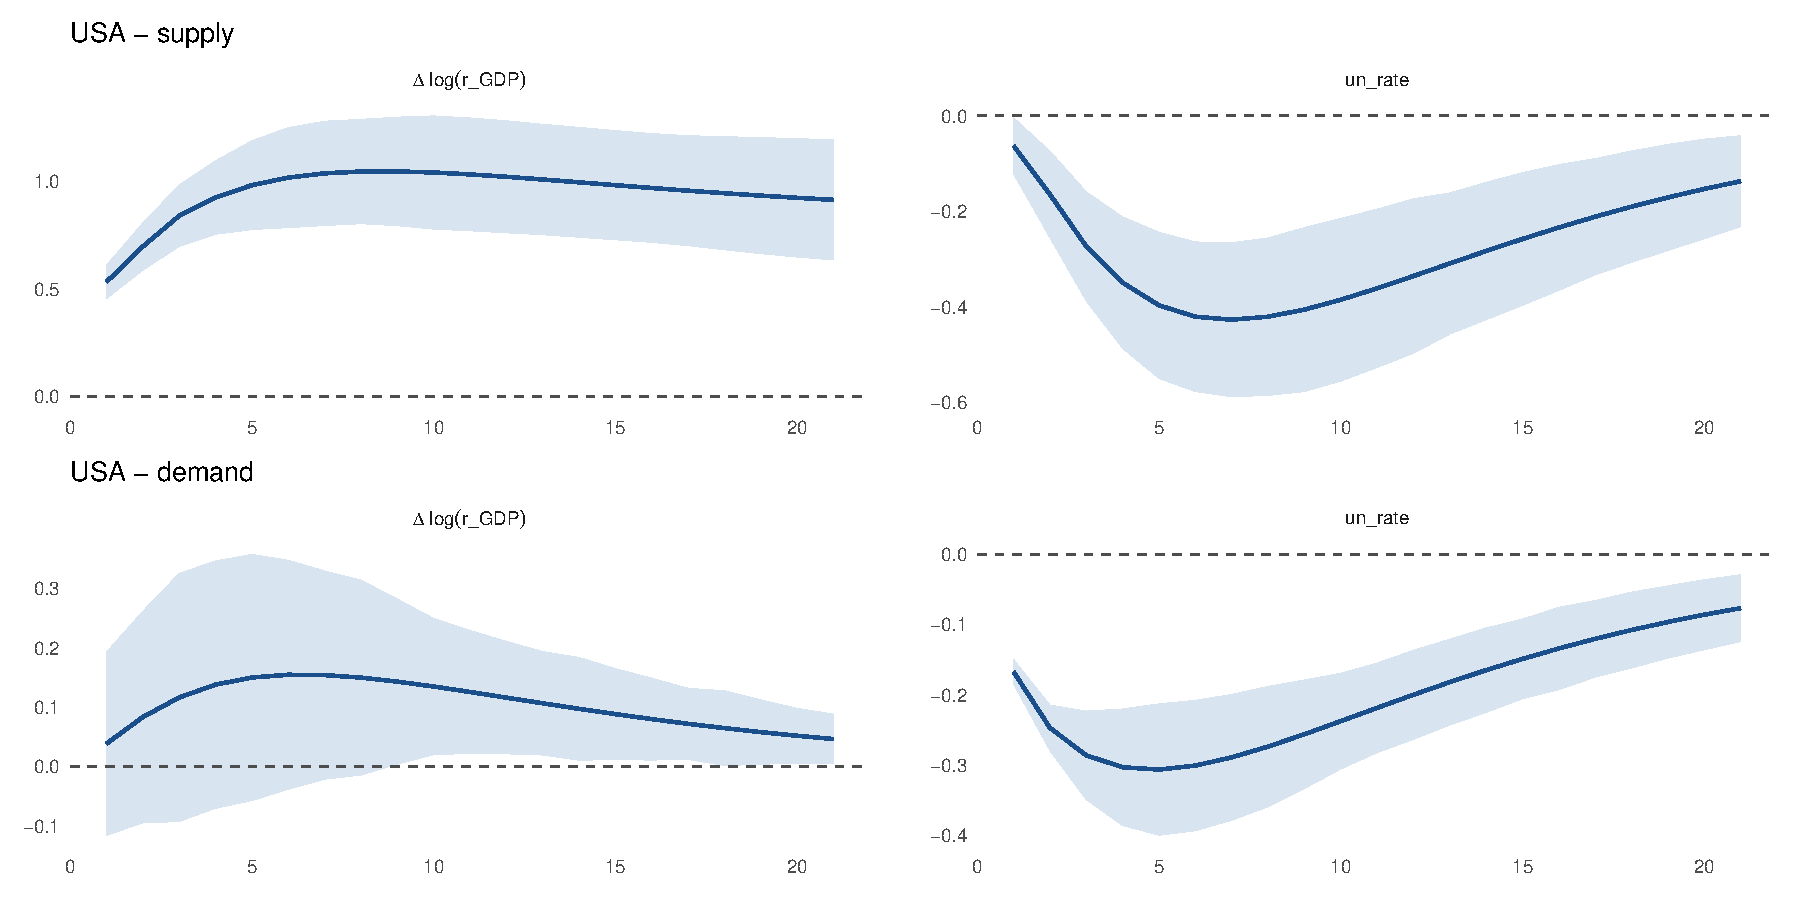
\includegraphics[width=0.9\textwidth]{Slides/USA_IRFs.pdf}
    \vspace{0.2cm} % Small vertical space
    \begin{minipage}{0.85\textwidth}
    \footnotesize
    Note: Upper - supply shock, bottom - demand shock, shaded areas are analytical (symmetric) 68\% confidence bands. Unemployment in levels. X-axis represents quarters.
    \end{minipage}
\end{center}
\end{frame}

\begin{frame}{Pairwise correlation - supply}
\setcounter{table}{0}
\label{main}
\begin{table}[H]
\captionsetup{justification=raggedright,
singlelinecheck=false
}
    \centering
    \scriptsize
    \caption{Pairwise correlations: supply shock.}  
    \begin{tabular}{l ccc ccc ccc c}
    \toprule
 & CAN & DKK & DEU & ESP & FRA & ITA & MEX & NOR & SWE & USA \\ 
  \hline
CAN & 1 &  &  &  &  &  &  &  &  &  \\ 
  DKK & -0.08 & 1 &  &  &  &  &  &  &  &  \\ 
  DEU & -0.24 & 0.14 & 1 &  &  &  &  &  &  &  \\ 
  ESP & -0.16 & 0.05 & 0.38 & 1 &  &  &  &  &  &  \\ 
  FRA & 0.07 & 0.08 & -0.25 & -0.22 & 1 &  &  &  &  &  \\ 
  ITA & -0.14 & 0.01 & 0.1 & -0.06 & 0.17 & 1 &  &  &  &  \\ 
  MEX & -0.19 & -0.13 & 0.4 & 0.2 & -0.08 & 0.15 & 1 &  &  &  \\ 
  NOR & 0.14 & 0.12 & -0.04 & 0 & -0.02 & 0.05 & 0.02 & 1 &  &  \\ 
  SWE & -0.04 & 0.14 & 0.31 & 0.25 & -0.01 & 0.1 & 0.02 & 0.13 & 1 &  \\ 
  USA & 0.02 & 0.17 & 0.09 & 0.22 & -0.08 & 0.07 & 0.18 & 0.03 & 0.12 & 1 \\ 
  \bottomrule
    \end{tabular}
    \begin{minipage}{\textwidth}
    \vspace{0.1cm} 
    \footnotesize Note: own summary, shocks are obtained using long-run restrictions. The period under analysis is 1990:Q2-2019:Q3 for all countries except Germany (1991:Q2-2019:Q3).
    \end{minipage}
    \label{table:a2}
\end{table}
\end{frame}

\begin{frame}{Pairwise correlation - demand}
    \begin{table}[H]
\captionsetup{justification=raggedright,
singlelinecheck=false
}
    \centering
    \scriptsize
    \caption{Pairwise correlations: demand shock.}
    \begin{tabular}{l ccc ccc ccc c}
    \toprule
 & CAN & DKK & DEU & ESP & FRA & ITA & MEX & NOR & SWE & USA \\ 
  \hline
CAN & 1 &  &  &  &  &  &  &  &  &  \\ 
  DKK & 0.2 & 1 &  &  &  &  &  &  &  &  \\ 
  DEU & 0.19 & 0.05 & 1 &  &  &  &  &  &  &  \\ 
  ESP & 0.12 & -0.03 & 0.1 & 1 &  &  &  &  &  &  \\ 
  FRA & 0.24 & 0.17 & 0.36 & -0.01 & 1 &  &  &  &  &  \\ 
  ITA & 0.14 & 0.2 & 0.14 & -0.07 & 0.28 & 1 &  &  &  &  \\ 
  MEX & 0.22 & 0.17 & 0.12 & 0.15 & 0.12 & 0.17 & 1 &  &  &  \\ 
  NOR & 0.13 & 0.23 & -0.11 & -0.02 & 0.13 & 0.14 & 0.1 & 1 &  &  \\ 
  SWE & 0.23 & 0.15 & 0.15 & -0.03 & 0.2 & 0.17 & 0.07 & 0.11 & 1 &  \\ 
  USA & 0.16 & 0.23 & 0.16 & -0.07 & 0.12 & 0.25 & 0.16 & 0.16 & 0.05 & 1 \\ 
    \bottomrule
    \end{tabular}
    \begin{minipage}{\textwidth}
    \vspace{0.1cm}
    \footnotesize Note: own summary, shocks are obtained using long-run restrictions. The period under analysis is 1990:Q2-2019:Q3 for all countries except Germany (1991:Q2-2019:Q3).
    \end{minipage}
    \label{table:a3}
\end{table}

 
\hfill \hyperlink{ortho}{\beamerbutton{Orthogonality}}    
 
\end{frame}


\begin{frame}{Methodology II - local projections}
We compute cumulative IRFs directly from local projections:
\begin{equation}
    y_{c,t+h} =  \beta^h z_{c,t} + \gamma^h_c + \gamma^h_t + \pi^h X_{c,t} + e^h_{c, t+h}
\label{eq:1}
\end{equation}
\noindent where $y_{c,t+h}$ is the log of Gini (total or subpopulation) for country $c$ measured at time $t+h$, $z_{c,t}$ is the exogenous shock, and $\beta^h$ are the estimated responses for $h = t+0,..,t+3$ periods after the shock. The remaining elements identify country fixed effects ($\gamma^h_c$) and time fixed effects ($\gamma^h_t$). 

\begin{itemize}
    \item Baseline $X_{c,t}$ includes two period lagged changes in inequality and exogenous shock used, i.e. supply or demand.
    \item For robustness $X_{c,t}$ includes: i) share of exports to the US (trade exposure), ii) changes in \textit{de facto} economic openness (proxied by the \textit{de facto} component of the KOF index), and iii) changes in domestic labor market policies (proxied by the Economic Freedom of the World's indicator of labor market regulation).
\end{itemize}
\end{frame}

% Results
\begin{frame}{Results I - baseline (unit change)}
\begin{figure}[H]
    \centering    
    \caption{Cumulative impulse responses to demand and supply shocks: Gini (total), baseline.}    
    \label{fig:demand_supply_base}
    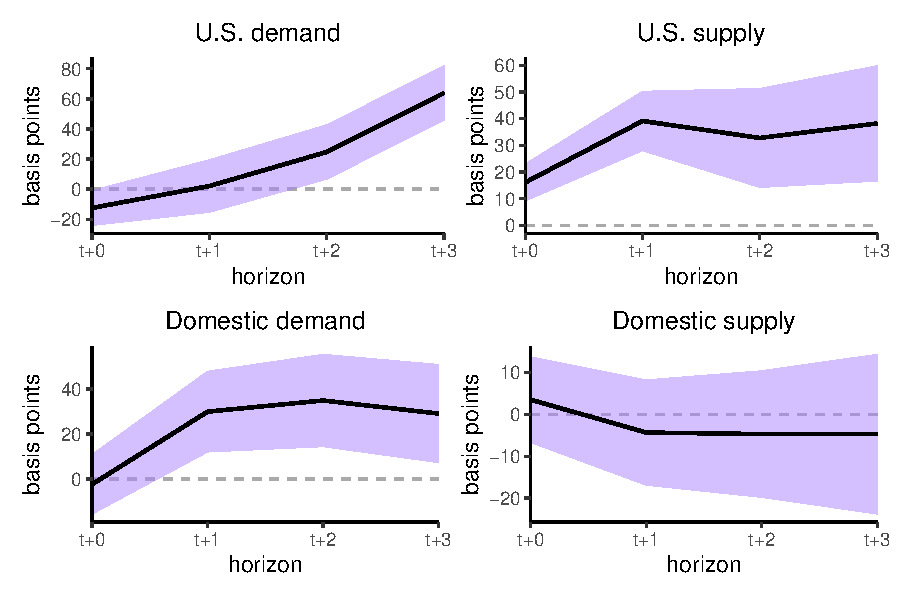
\includegraphics[width=0.60\textwidth]{Figures/baseline_demand_supply_LP_extended.pdf}
    \centering \caption*{Note: percentages in decimals, shaded areas represent 68\% Driscoll-Kraay confidence bands.}
\end{figure}
\end{frame}

\begin{frame}{Results II - gender (unit change)}
\begin{figure}[H]
    \centering    
    \caption{Cumulative impulse responses to demand and supply shocks: Gini (by gender), baseline.}    
    \label{fig:demand_supply_gender_base}
    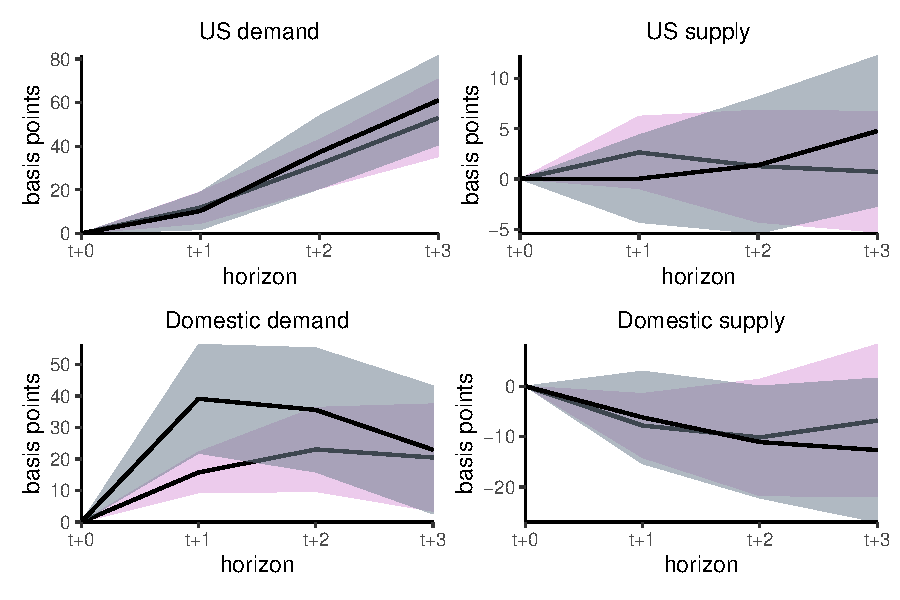
\includegraphics[width=0.55\textwidth]{Figures/baseline_gender_LP_extended.pdf}
    \centering \caption*{Note: percentages in decimals, men's IRF is presented in gray, women's IRF is presented in pink.}
\end{figure}
\end{frame}

\begin{frame}{Results III - robustness (unit change, total)}
\begin{figure}[H]
    \centering
    \caption{Cumulative impulse responses to demand and supply shocks: Gini (total), robustness.}
    \label{fig:demand_supply_robust}
    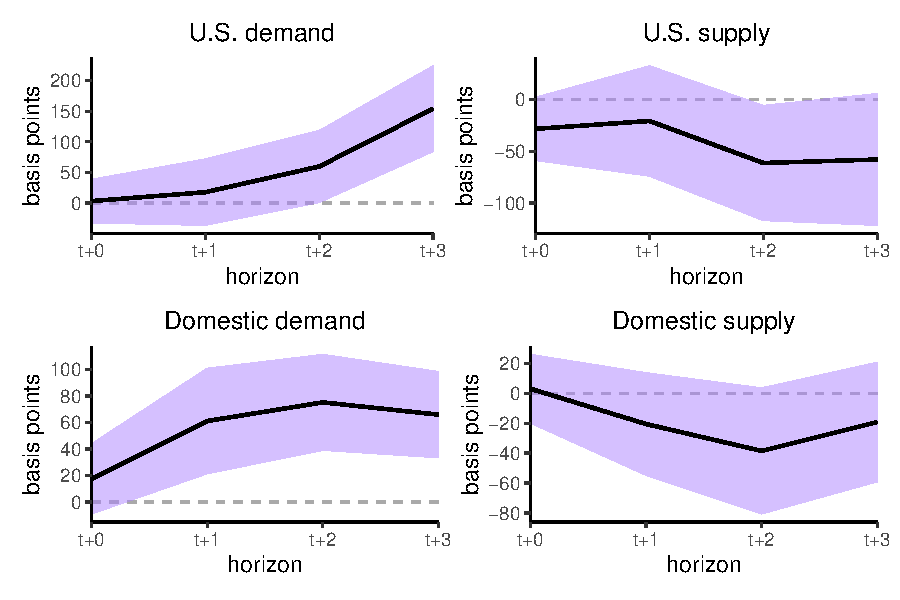
\includegraphics[width=0.60\textwidth]{Figures/robust_demand_supply_LP_extended.pdf}
    \centering \caption*{Note: percentages in decimals, shaded areas represent 68\% Driscoll-Kraay confidence bands.}
\end{figure}   
\end{frame}

% Conclusion

\begin{frame}{Interpretation and discussion I}
    \begin{itemize}
        \item<1-> \textbf{Demand shocks}. We interpret the significant impact of changes in US demand using the fact that changes in employment cause changes in income and current consumption. We think that US consumption of foreign goods and services is one of the important drivers behind inequality abroad.

        \begin{itemize}
            \item<2-> US demand shock $\rightarrow$ $\uparrow$ US employment \& consumption $\rightarrow$ $\uparrow$ inequality abroad
            \item<3-> US supply shock $\rightarrow$ $\uparrow$ US employment \& consumption $\rightarrow$ $\uparrow$ inequality abroad — but the link is weaker and not persistent?
        \end{itemize}
        
        \item<4-> \textbf{Supply shocks}. Are not as persistent, but generally tend to reduce inequality.
    \end{itemize}
\end{frame}

\begin{frame}{Interpretation and discussion II}
    \begin{itemize}
        \item<1-> \textbf{US vs domestic shocks}. The magnitude of the cumulative shock impact is linked to US purchasing power and economic scale.
        \item<2-> \textbf{Gender}. Similar pattern to total Gini with a bit of a gap between males and females (domestic demand shock): income inequality appears to grow faster for men, than for women (probably due to the variability in earnings among men).
        \item<3-> \textbf{Exposure to shocks}. Our sample features relatively strong economic links with the US, so the results could potentially be lower in a more dispersed sample.
    \end{itemize}
\end{frame}


% End page--------------------------------------------------------------------
\begin{frame}
\begin{center}
\begin{Large}
\vspace{10pt}
Thank you! 
\end{Large}


\includegraphics[width=0.5\textwidth]{Slides/logo_solo.png}

\begin{Large}
\vspace{10pt}
Questions or suggestions? 
\end{Large}
\end{center}
\bigskip


\alert{w}:\hspace{9pt}grape.org.pl \\
\alert{t}:\hspace{12pt}grape\_org \\
\alert{f}:\hspace{12pt}grape.org \\
\alert{e}:\hspace{11pt}o.gurshev@grape.org.pl
\end{frame}

\begin{frame}{Appendix - shock orthogonality}
\setcounter{table}{0}
\label{ortho}
\begin{table}[H]
\captionsetup{justification=raggedright,
singlelinecheck=false
}
    \centering
    \caption{Correlation coefficients (within country) between supply and demand shocks.}
    \begin{tabular}{l ccc ccc ccc cc}
    \toprule
 

	Country&	CAN	&	DKK	&	DEU	&	ESP	&	FRA	&	ITA	&	MEX	&	NOR	&	SWE	&	USA	\\    \midrule
Correlation	&	0	&	0	&	0	&	0	&	0	&	0	&	0	&	0	&	0	&	0	\\

    \bottomrule
    \end{tabular}
    \begin{minipage}{\linewidth}
    \footnotesize
    \centering
    Note: Pearson correlation.
    \end{minipage}
\end{table}
\hyperlink{main}{\beamerbutton{Back to main slides}}
\hyperlink{disturb}{\beamerbutton{US shocks graphs}}
\end{frame}


\begin{frame}{Appendix - disturbances}
\label{disturb}
    \begin{center}
        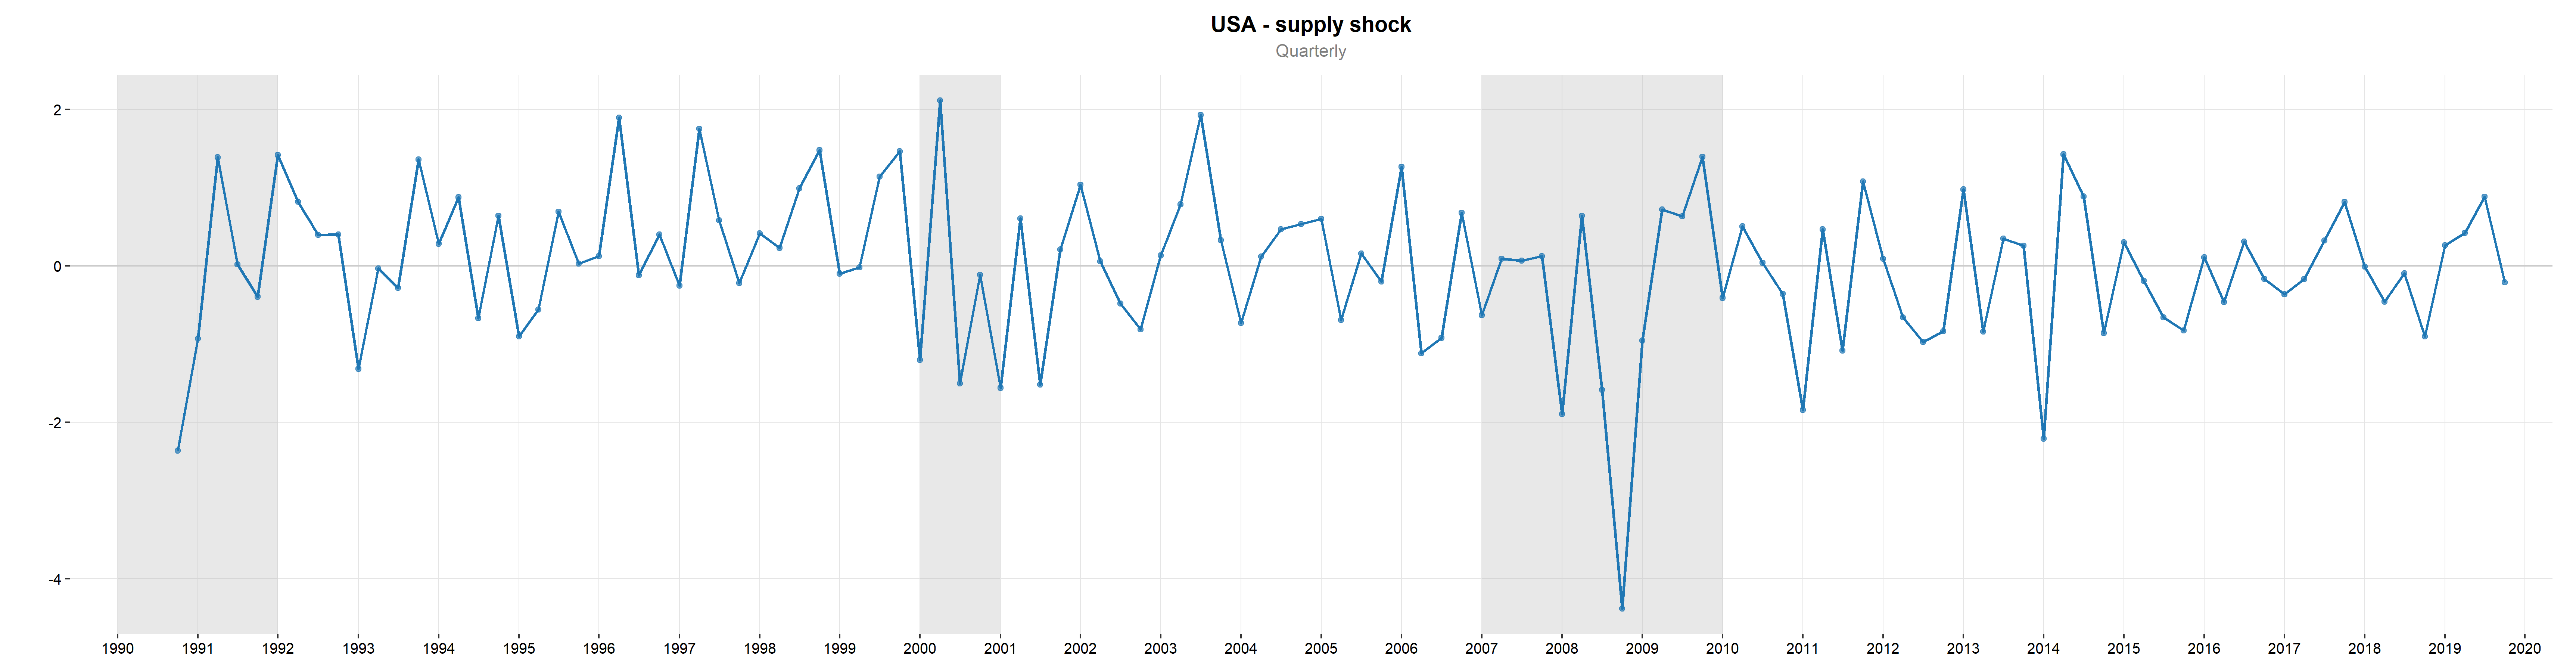
\includegraphics[width=0.82\textwidth]{Slides/usa_gdp_shocks.png}
        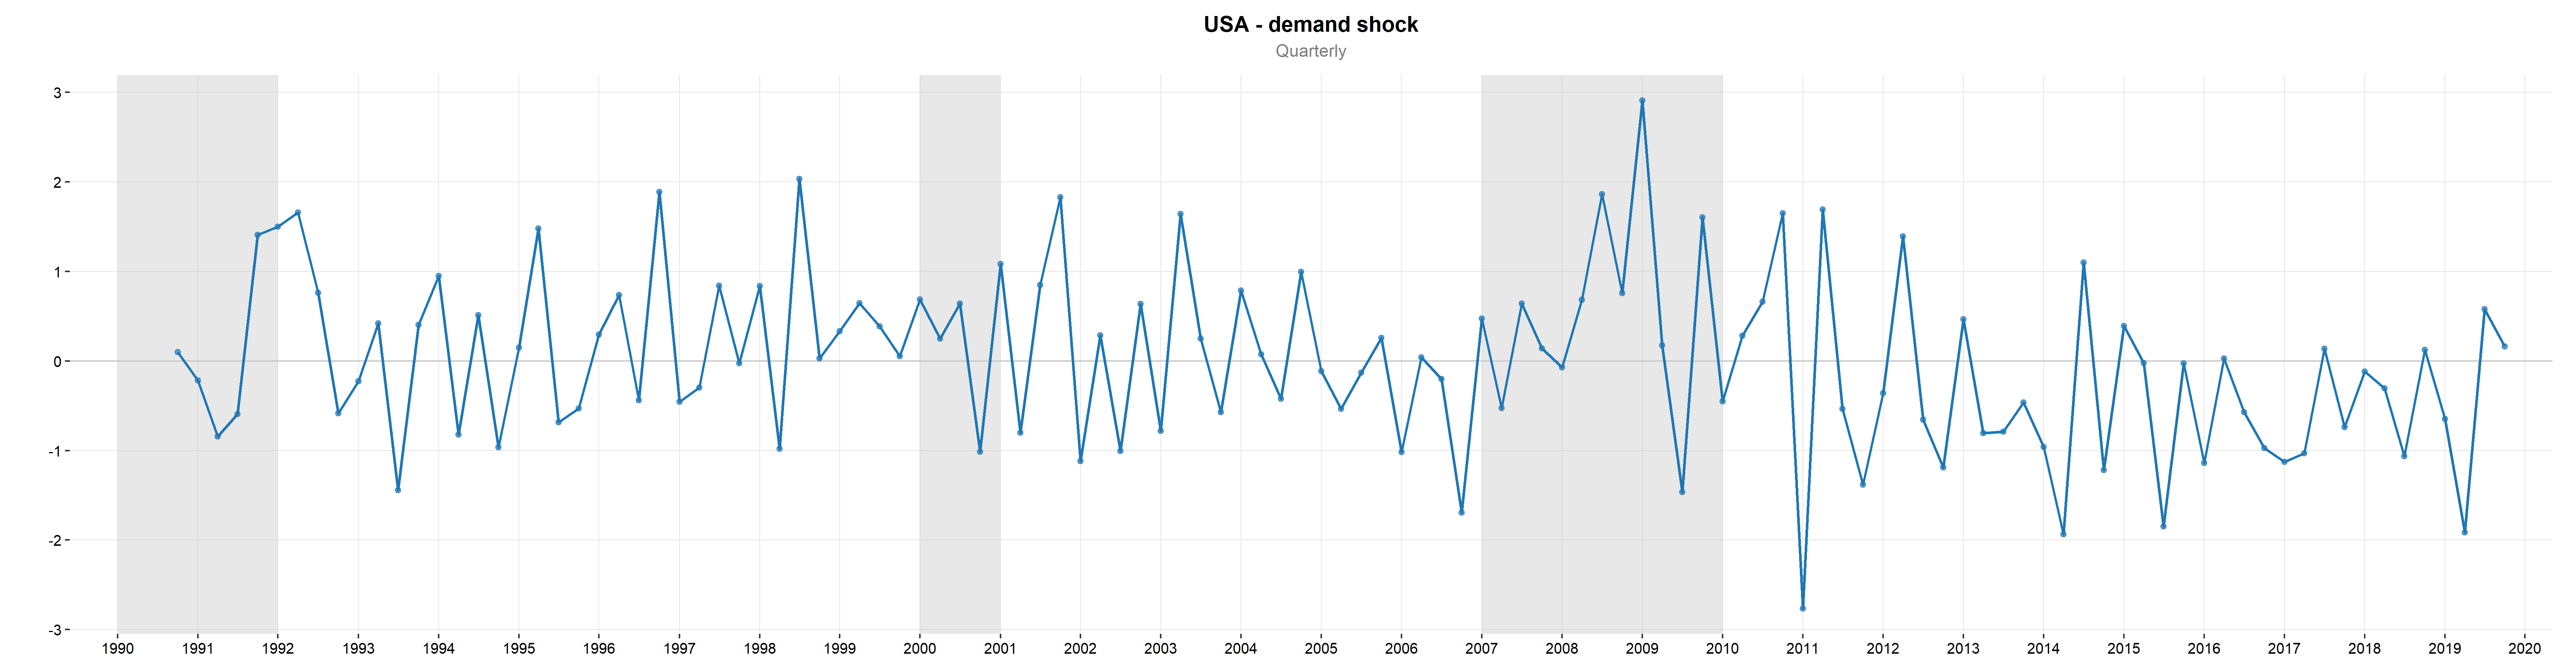
\includegraphics[width=0.82\textwidth]{Slides/usa_unemp_shocks.png}
    \begin{minipage}{0.85\textwidth}
    \footnotesize
    Note: Shaded areas are NBER recessions.
    \end{minipage}
    \end{center}
\hfill  \hyperlink{main}{\beamerbutton{back to main slides}}
\end{frame}

\begin{frame}{Appendix - long-run restrictions}
\label{LRvar}
\footnotesize
\textbf{VAR:}
\begin{align*}
Y_t &= A_1 Y_{t-1} + A_2 Y_{t-2} + \cdots + A_p Y_{t-p} + u_t
\end{align*}

\textbf{MA form:}
\begin{align*}
Y_t &= C(L) u_t = \sum_{i=0}^\infty C_i u_{t-i}
\end{align*}

\textbf{Structural form:}
\begin{align*}
Y_t &= B(L) \varepsilon_t = \sum_{i=0}^\infty B_i \varepsilon_{t-i}
\end{align*}

\textbf{Long-run restriction:}
\begin{align*}
u_t = S \varepsilon_t, \quad C(\infty) S = B(\infty), \quad 
\left[ B(\infty) \right]_{1,2} = 0
\end{align*}

\textbf{Impact matrix:}
\begin{align*}
\Sigma_u = SS' \quad \text{(covariance of reduced-form residuals)}
\end{align*}

\hfill \hyperlink{VAR}{\beamerbutton{Back to main slides}}
\end{frame}


\begin{frame}[allowframebreaks]
\bibliographystyle{apalike}
\bibliography{Slides/slides_bibliography}
\end{frame}
\end{document}